\subsection{Distributed computing infrastructure}

% CHEP12 "Trying to Predict the Future - Resource Planning and Allocation
% in CMS" P. Kreuzer
% https://cms-mgt-conferences.web.cern.ch/cms-mgt-conferences/conferences/pres_display.aspx?cid=665&pid=4582

% CHEP10 "Experience with the CMS Computing Model from commissioning to
% collisions" D. Bonacorsi
% https://cms-mgt-conferences.web.cern.ch/cms-mgt-conferences/conferences/pres_display.aspx?cid=462&pid=2306

% CHEP10 "Monitoring the Readiness and Utilization of the Distributed CMS
% Computing Facilities during the first year LHC running" J. Hernandez
% https://cms-mgt-conferences.web.cern.ch/cms-mgt-conferences/conferences/pres_display.aspx?cid=462&pid=2332
% Note that we don't currently have monitoring in here as an explicit
% topic.  But it probably needs to be discussed in operations, at the very least.

% CHEP10 "CMS Distributed Computing Integration in the LHC sustained
% operations era" C. Grandi
% https://cms-mgt-conferences.web.cern.ch/cms-mgt-conferences/conferences/pres_display.aspx?cid=462&pid=2264

From the very start, CMS planned on having a distributed computing
infrastructure.  While HEP collaborations have historically relied on a
single large computational resource located at the host laboratory for
virtually all of their data processing and storage needs, and while a
single facility would have ultimately been more efficient to operate, it
was not considered feasible to ask the nations of the LHC experimental
collaborations to contribute funds for a computing center at CERN.
Instead, each nation has established domestically owned and operated sites
that contribute to the LHC experiments' computing needs.  These sites,
distributed around the world, have given greater prominence to the LHC
experiments within their participating nations, which has led to greater
funding and more engagement from local computing experts, who would not
have had a chance to participate had all the computing been done at CERN.
CMS has successfully leveraged this local expertise to improve the
experiment's computing systems and their operation.

The CMS distributed computing infrastructure is a tiered set of computing
sites connected through networks that follows the MONARC
model~\cite{MONARC}. The computing infrastructure is organized in a
hierarchy starting with CERN at its origin called Tier 0 (T0).  On the next
level, seven regional computing centers called Tier-1 (T1) sites form the
backbone of the system, followed by Tier-2 (T2) and Tier-3 (T3) sites at
universities and/or research institutes.  

Sites at each tier in the hierarchy are responsible for performing certain
workflows, and the sites are configured to support those particular
workflows.  The T0 site is responsible for data recording and first-pass
(``prompt'') data reconstruction, and also for performing calibrations that
are needed for the reconstruction.  Prompt reconstruction starts 48 hours
after events have been recorded to incorporate updated calibrations.  The
production of calibration constants is described in
Section~\ref{sec:constants}.  All events are stored in the RAW format on
tape at the T0 site.  \fixme{We'll need to be sure that RAW etc. are
  defined earlier on; this sounds like software.}  The T0 facility thus
needs substantial processing and storage resources.  At the end of Run 1,
the CMS T0 facility had \fixme{Get all the T0 parameters!}.

The primary workflows at T1 sites are the simulation of events and the
re-reconstruction of both detector and simulation events.  Simulation is a
processing-intensive workflow, requires little or no input data, but has
large output data.  Re-reconstruction of the data and simulation samples is
performed when changes to reconstruction algorithms and/or calibrations are
sufficiently different from those of the prompt reconstruction to have a
significant impact on understanding the physics of the LHC collisions.  The
re-reconstruction workflow also requires substantial processing resources,
and both the input and output data sizes are large.  In addition, the T1
sites are responsible for maintaining a second archived copy of the data in
RAW format, so that between the T0 and T1 sites, there are two tape copies
of every event.  CMS operated seven T1 sites during Run 1, hosted by
Germany, Spain, France, Italy, Taiwan, the United Kingdom and the United
States.  At the end of the run, the aggregated Tier 1 resources were
\fixme{Get all the T1 parameters!  Do we discuss relative sizes of sites?
  Mention the hosting institutions?}

T2 sites are also responsible for some simulation workflows, and also for
analysis of data and simulation samples by physics users; no user analysis
takes place at T0 or T1.  The input datasets for analysis is distributed to
the sites in advance, and then jobs seeking to analyze a particular dataset
are sent to a site that hosts the data.  While the input data for analysis
is typically large, the output is usually several orders of magnitude
smaller, as users reduce and refine the data to meet their specific
interests and needs.  \fixme{Give some typical sizes for these?  Does such
  a thing exist?}  T2 sites do no archival storage, so are only required to
deploy disk and processing resources.  In Run 1, there were about fifty T2
sites, which in aggregate provided \fixme{Get all the T2 parameters!}.

An important distinction between T2 sites and those at T0 and T1 is that
the latter were used by a small number of operators for centrally-organized
production tasks.  The T2 sites were used by physicists throught the
collaboration in a ``chaotic'' mode.  Thousands of users might submit jobs
to any given site.  To maintain scalability of management, users do not
directly log in to computers at the sites, but instead submit jobs through
grid technologies~\cite{thegrid}.  A computing grid is an infrastructure
that allows different administrative domains to share access to services,
processors and storage with a select set of users and groups of users. The
computing sites that are members of a grid provide a uniform environment
for user batch jobs, even if each cluster has some unique local
configuration.  As a result, any user job can, in principle, be executed at
any site on the grid with little user customization required.  Users of the
grid resources are issued credentials that can be attached to a batch job
when it is submitted to a resource; these credentials allow for the
tracking of jobs back to individual users.  CMS sites operated using three
different grid technologies.  [NOW HERE -- cite EGI, OSG and ARC.]

All sites are interconnected via
dedicated or general purpose scientific networks. The original design
separated the T2 sites into groups that were associated and connected
to only one T1. During LHC Run 1, the strength and reliability of the
networks allowed for a more flexible setup, realizing a full-mesh network
topology where every T2 site is connected to every T1 site and
every other T2 site, as shown in Figure~\ref{fig:distributed_topology}.

\begin{figure}
\begin{center}
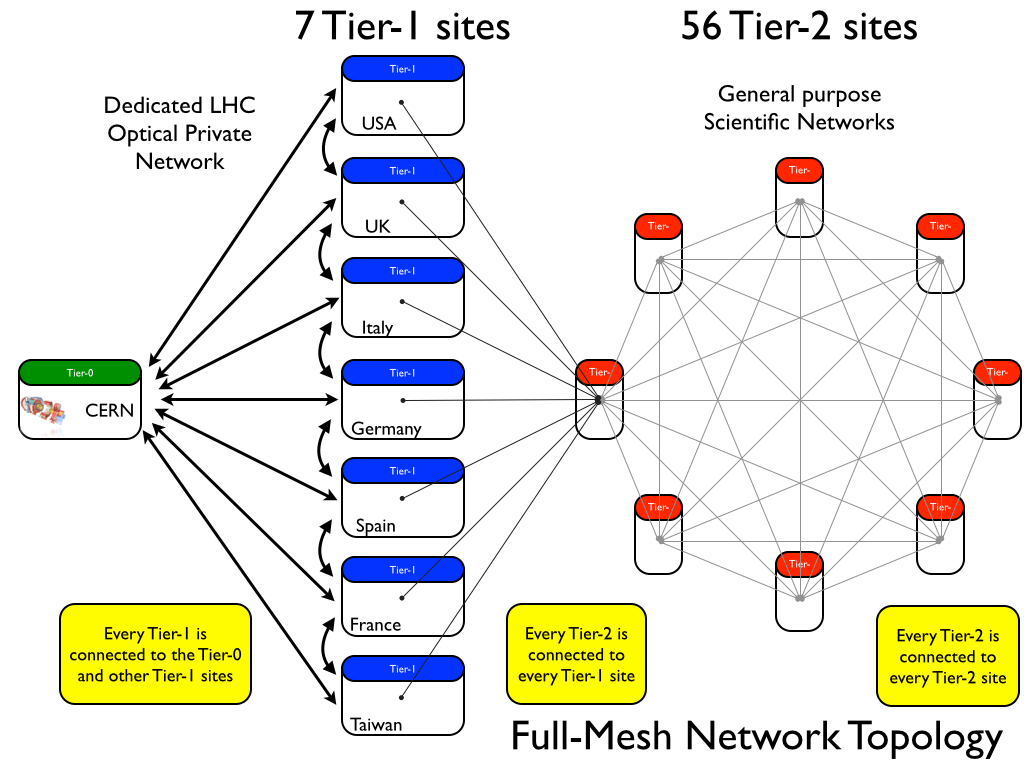
\includegraphics[width=.5\textwidth]{figs/distributed_topology}
\end{center}
\caption{The tiered CMS computing infrastructure showing the Tier-0, Tier-1 and Tier-2 levels interconnected with dedicated or general purpose scientific networks in a full-mesh network topology.
  \label{fig:distributed_topology}}
\end{figure}

T1 sites provide access to large CPU farms and a mass storage system
(MSS) with disk caches and tape libraries. They are different from T2
sitess in two main aspects. T1 sites provide continuous (``24/7'')
support operation, while T2 sites are operated during business hours
and unattended in between. In addition, T2 sites do not have tape
libraries at the sites and operate purely with disk caches.  T3 sites
are owned and managed by individual institutes, at a support level of their
choosing.

The network between the sites is the backbone of the CMS computing
infrastructure, as its operation relies on transferring files among the
sites for access. The network between the T0 and T1 sites is the dedicated
LHC Optical Private Network (LHCOPN).~\fixme{Does this get a
  reference?}. The T2 sites are connected through general purpose
scientific networks in their host countries. The main data flows can be
separated into archiving and serving. Archiving is tape based where related
files are grouped by physics content on separate sets of tape cartridges
(known as tape families) to optimize writing, recall, and
recycling. Serving is disk based. The main data flows are as follows:
